% Plant Disease Classification - technical report
% Compiles with pdfLaTeX on Overleaf. No non-standard packages.

% 10pt with 2.5cm margins rather than 11pt/2.1cm: the same content, a page and a
% half shorter, and the wider margin keeps the line length readable at the smaller
% size. Nothing was cut to hit the page budget.
\documentclass[10pt,a4paper]{article}

\usepackage[margin=2.5cm]{geometry}
\usepackage[T1]{fontenc}
\usepackage{lmodern}
\usepackage{graphicx}
\usepackage{booktabs}
\usepackage{xcolor}
\usepackage{caption}
\usepackage{subcaption}
\usepackage{enumitem}
\usepackage{float}
\usepackage{tikz}
\usetikzlibrary{arrows.meta,positioning,fit,backgrounds}
\usepackage[colorlinks=true,linkcolor=black,citecolor=black,urlcolor=accent]{hyperref}

\definecolor{accent}{HTML}{2F6F43}
\definecolor{diseased}{HTML}{A8442A}
\graphicspath{{figures/}}

% ---------------------------------------------------------------------------
% Deployed URLs. Paste them in here after deploying and recompile; the callout
% under the title switches from "not yet live" to a highlighted link on its own.
% ---------------------------------------------------------------------------
\def\dashboardurl{}
\def\apiurl{}

% Shared node styles for the two diagrams.
\tikzset{
  pipebox/.style={draw=gray!55,rounded corners=2pt,fill=white,align=center,
                  minimum height=8mm,inner xsep=3pt,inner ysep=2pt,font=\scriptsize},
  trainbox/.style={pipebox,draw=accent!55,fill=accent!8},
  servebox/.style={pipebox,draw=diseased!45,fill=diseased!6},
  flow/.style={-{Stealth[length=1.7mm]},gray!75,semithick},
}

\captionsetup{font=small,labelfont=bf}
\setlist{nosep,leftmargin=1.4em}
\setlength{\parskip}{0.35em}
\setlength{\parindent}{0pt}

\title{\vspace{-1.4cm}\textbf{Plant Disease Classification}\\[0.25em]
\large A binary healthy/diseased leaf classifier, from dataset audit to deployment}

\author{Krithick Balaji Ramesh}
\date{August 2026}

\begin{document}
\maketitle
\vspace{-1.1cm}

\begin{center}\small
\href{https://www.linkedin.com/in/krithick-balaji-ramesh-546245255}{LinkedIn} \,$\cdot$\,
\href{https://ramesh-profile.vercel.app}{Portfolio} \,$\cdot$\,
\href{https://iias-krithick.vercel.app}{Research Profile} \,$\cdot$\,
\href{https://scholar.google.com/citations?hl=en\&user=eJ23GcwAAAAJ}{Google Scholar} \,$\cdot$\,
\href{https://github.com/Krithii06}{GitHub}
\end{center}

\begin{center}
\ifx\dashboardurl\empty
  \small\textcolor{gray!75}{Live dashboard: not yet deployed at the time of writing ---
  see Section~\ref{sec:deployment}.}
\else
  \setlength{\fboxsep}{7pt}%
  \fcolorbox{accent}{accent!10}{%
    \parbox{0.66\textwidth}{\centering
      \textbf{\href{\dashboardurl}{\textcolor{accent}{View the live dashboard}}}\\[0.15em]
      \scriptsize\texttt{\dashboardurl}}}
\fi
\end{center}

\vspace{0.2em}
\hrule
\vspace{0.8em}

\section*{Abstract}

This report documents a binary healthy/diseased classifier for apple leaf images,
trained on a four-class subset of PlantVillage and served through a FastAPI endpoint
with a React front end. The model reaches \textbf{99.51\% accuracy} and
\textbf{0.9951 macro F1} on a held-out test set of 611 images.

That number is not the interesting part. PlantVillage photographs each physical leaf
several times, and the 3{,}171 images used here come from only \textbf{505 distinct
leaves}. Splitting them at random puts near-identical photographs of the same leaf on
both sides of the split. Measured directly, a naive random split leaves \textbf{100\%}
of validation images with a photograph of the same leaf in training, against
\textbf{0\%} for the leaf-grouped split used throughout. Most of the design below
follows from taking that seriously, and the reported figure is the one that survives it.

\section{Problem and scope}

The task is to classify a plant leaf photograph by health condition and present the
prediction through a web interface, using PlantVillage, a CNN or transfer-learning
model, accuracy/precision/recall/F1 with a confusion matrix, and free hosting with a
public URL.

\textbf{An ambiguity in the brief.} The class selection is specified twice and the two
statements disagree: one section asks for ``3--5 suitable classes\ldots at least one
representing a healthy condition'', the task list for ``only two classes: (Healthy,
Diseased)''. Rather than pick a reading silently, this project satisfies both --- four
source classes (three apple diseases plus apple healthy), mapped onto a binary target
for the deployed model. Evaluation reports the binary metrics and breaks them down by
the four source diseases, which is where the informative errors turn out to be.

\section{Dataset}

PlantVillage \cite{mohanty2016} contains 54{,}305 images across 38 classes and 14 crop
species, licensed CC BY-SA 3.0. Counted from the official split files the total is
54{,}305, not the 54{,}306 quoted on the dataset card --- a one-image discrepancy, noted
for accuracy and of no consequence. Imbalance across the full dataset is severe:
5{,}507 images in the largest class against 152 in the smallest, about 36 to one, which
is one reason a single crop was selected rather than all of it.

The four apple classes were chosen for three reasons. First, every apple image resolves
to a real entry in the dataset's leaf-grouping map --- 3{,}171 of 3{,}171, no fallbacks.
Apple is the only crop for which this holds, and since the argument of this report rests
on grouping images by physical leaf, the grouping had to be verifiable rather than
assumed. Second, the binary target is nearly balanced at 51.9\% healthy, so accuracy is
a meaningful headline number and no class weighting is needed. Third, four classes with
one healthy class matches the brief's stated range directly.

\begin{table}[H]
\centering\small
\caption{Selected subset and the binary target it collapses into.}
\begin{tabular}{lrl}
\toprule
\textbf{Source class} & \textbf{Images} & \textbf{Binary label} \\
\midrule
\texttt{Apple\_\_\_Apple\_scab}        & 630   & diseased \\
\texttt{Apple\_\_\_Black\_rot}         & 621   & diseased \\
\texttt{Apple\_\_\_Cedar\_apple\_rust} & 275   & diseased \\
\texttt{Apple\_\_\_healthy}            & 1{,}645 & healthy \\
\midrule
\textbf{Total} & \textbf{3{,}171} & 1{,}645 healthy / 1{,}526 diseased \\
\bottomrule
\end{tabular}
\end{table}

\textbf{What was actually checked.} The subset was profiled before training rather than
assumed clean. All 3{,}171 files are 256$\times$256, RGB and JPEG; none failed to decode.
MD5 found seven byte-identical pairs and a 64-bit difference hash seven near-duplicate
pairs at Hamming distance $\leq 3$ --- every one of them inside a single leaf group, so
the grouped split handles them and nothing was discarded. Resolution is reported as a
sentence rather than a histogram, because every file is the same size.

\subsection*{How the system works end to end}

The project splits into an offline half that produces a model and an online half that
serves it. The only thing crossing between them is the exported bundle --- ONNX graph,
class mapping, preprocessing settings --- which is why the serving image needs no PyTorch.

\begin{figure}[H]
\centering
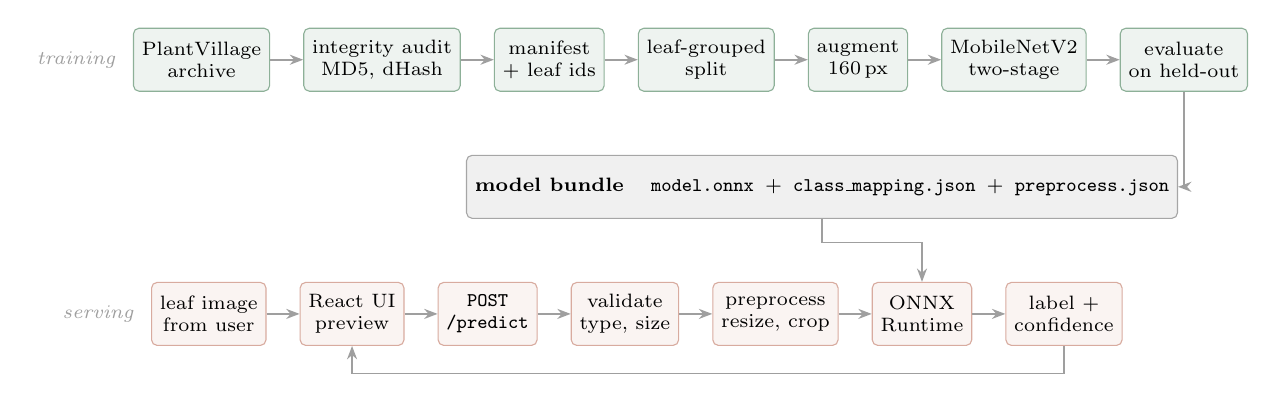
\begin{tikzpicture}[node distance=3.6mm and 4.2mm]

% --- offline: dataset to exported model ---
\node[trainbox] (raw)    {PlantVillage\\archive};
\node[trainbox, right=of raw]   (audit)  {integrity audit\\MD5, dHash};
\node[trainbox, right=of audit] (man)    {manifest\\+ leaf ids};
\node[trainbox, right=of man]   (split)  {leaf-grouped\\split};
\node[trainbox, right=of split] (aug)    {augment\\160\,px};
\node[trainbox, right=of aug]   (train)  {MobileNetV2\\two-stage};
\node[trainbox, right=of train] (eval)   {evaluate\\on held-out};

\foreach \a/\b in {raw/audit, audit/man, man/split, split/aug, aug/train, train/eval}
  \draw[flow] (\a) -- (\b);

% --- the artefact that crosses the boundary ---
\node[pipebox, draw=gray!70, fill=gray!12, below=8mm of split.south east, xshift=6mm]
  (bundle) {\textbf{model bundle} \;\; \texttt{model.onnx} \,+\, \texttt{class\_mapping.json}
            \,+\, \texttt{preprocess.json}};
\draw[flow] (eval.south) |- (bundle.east);

% --- online: upload to answer ---
\node[servebox, below=8mm of bundle.south west, anchor=north west, xshift=-40mm] (user) {leaf image\\from user};
\node[servebox, right=of user]  (ui)    {React UI\\preview};
\node[servebox, right=of ui]    (post)  {\texttt{POST}\\\texttt{/predict}};
\node[servebox, right=of post]  (valid) {validate\\type, size};
\node[servebox, right=of valid] (prep)  {preprocess\\resize, crop};
\node[servebox, right=of prep]  (ort)   {ONNX\\Runtime};
\node[servebox, right=of ort]   (out)   {label +\\confidence};

\foreach \a/\b in {user/ui, ui/post, post/valid, valid/prep, prep/ort, ort/out}
  \draw[flow] (\a) -- (\b);
\draw[flow] (bundle.south) -- ++(0,-3mm) -| (ort.north);
\draw[flow] (out.south) -- ++(0,-3.5mm) -| (ui.south);

\node[font=\scriptsize\itshape, gray!75, left=1mm of raw]  {training};
\node[font=\scriptsize\itshape, gray!75, left=1mm of user] {serving};

\end{tikzpicture}
\caption{End-to-end workflow. The top row runs once on a laptop CPU and ends in an
exported bundle; the bottom row is what a request actually touches. The bundle is the
only coupling between them.}
\label{fig:pipeline}
\end{figure}

\section{Splitting, and the leakage it avoids}

The test set is PlantVillage's own held-out split, left untouched and used once, after
model selection had finished on validation. Validation is carved out of the official
training portion with \texttt{StratifiedGroupKFold} grouped on leaf identity and
stratified on the four source classes, so that cedar apple rust --- the rarest disease,
275 images --- stays represented. The split is seeded and reproducible, and the test
suite asserts that no leaf appears in more than one split.

The official split was audited rather than trusted: no leaf group spans its train/test
boundary, for the apple subset or for the dataset as a whole. That is why it is used
as the test set here.

\begin{table}[H]
\centering\small
\caption{Final splits. Leaf counts matter more than image counts.}
\begin{tabular}{lrrrr}
\toprule
\textbf{Split} & \textbf{Images} & \textbf{Leaves} & \textbf{Healthy} & \textbf{Diseased} \\
\midrule
train & 2{,}131 & 340 & 1{,}131 & 1{,}000 \\
val   & 429     & 68  & 228     & 201 \\
test  & 611     & 97  & 286     & 325 \\
\bottomrule
\end{tabular}
\end{table}

\begin{figure}[H]
\centering
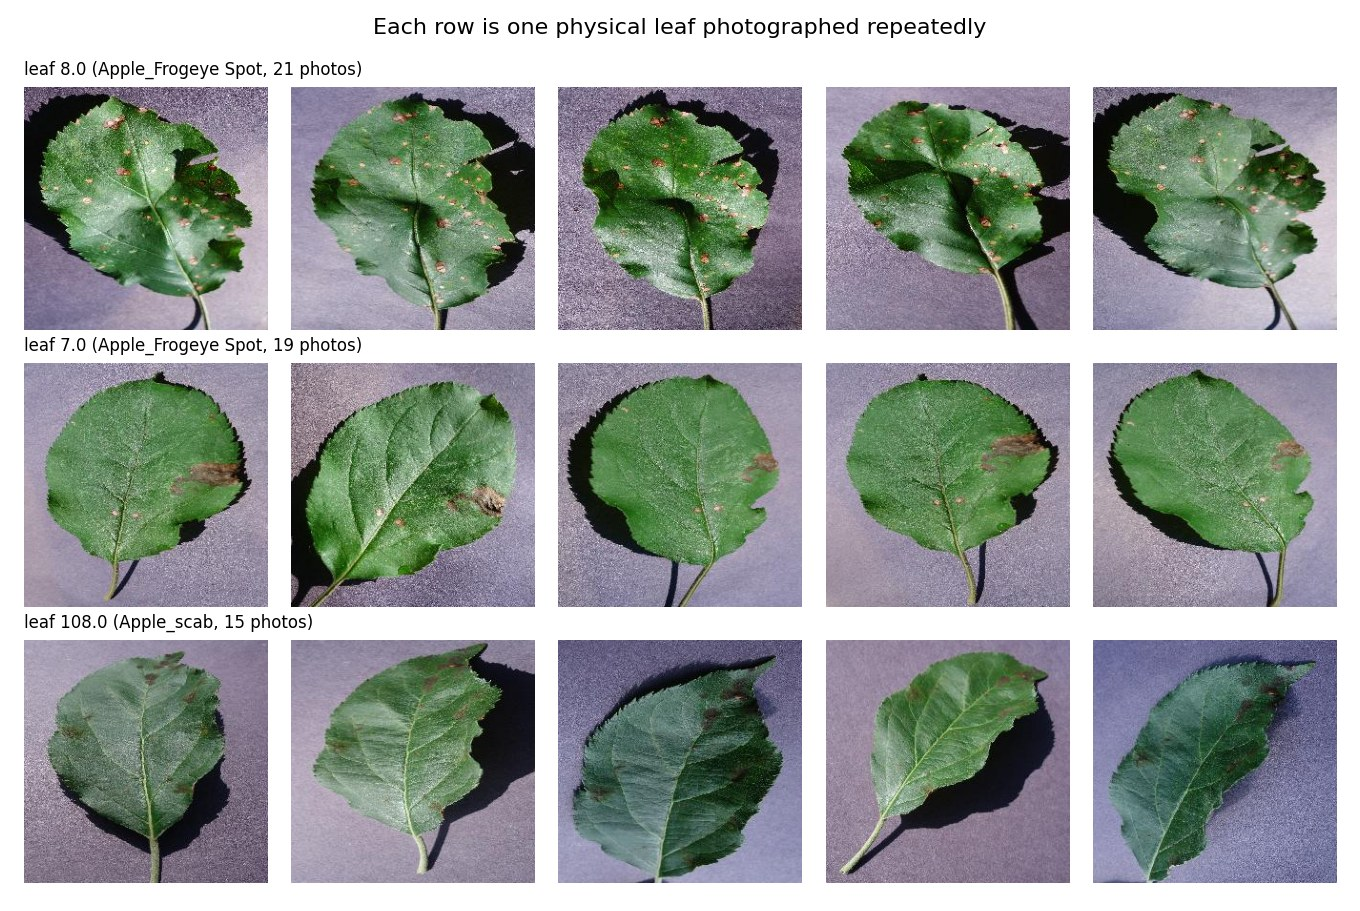
\includegraphics[width=0.60\textwidth]{leaf_groups.jpg}
\caption{Each row is one physical leaf, photographed repeatedly from different angles.
A random image split scatters these rows across train and test.}
\end{figure}

\textbf{Measuring the leak.} The cost of splitting on images rather than leaves was
measured directly, without training anything, by counting how many held-out images have
a photograph of the same physical leaf in training.

\begin{table}[H]
\centering\small
\caption{Structural leakage. Two of the naive split's leaked pairs are byte-identical
duplicates.}
\begin{tabular}{lrrr}
\toprule
\textbf{Split strategy} & \textbf{Val images} & \textbf{Sharing a leaf with train} & \textbf{Share} \\
\midrule
Leaf-grouped (used here)  & 429 & 0   & 0.0\%   \\
Naive random image split  & 426 & 426 & 100.0\% \\
\bottomrule
\end{tabular}
\end{table}

A structural measure is used in preference to an accuracy comparison, and the reason is
worth stating plainly. The binary apple task saturates --- validation macro F1 reaches
1.0000 by the third epoch --- so an accuracy gap between the two strategies would
understate the problem, because there is no headroom in which the optimism can show
itself. A second model was trained on the naive split to confirm that, and it is
reported alongside the others in Section~6: it lands within one image of the grouped
run, which is noise rather than a finding. The leak is present regardless, and the count
above does not depend on the model being weak enough to reveal it.

\section{Preprocessing and augmentation}

Training images get a random resized crop to 160 pixels at scale 0.7--1.0, horizontal
and vertical flips, rotation up to 20 degrees, and mild colour jitter. Validation, test
and production inputs share one deterministic path: resize the shorter side to 182,
centre crop to 160, normalise with ImageNet statistics.

Two choices need justifying. \textbf{Both flips are enabled} --- these are detached
leaves on a plain background, so there is no canonical orientation and mirroring is a
realistic variation rather than a distortion. This would not be safe for imagery where
gravity or plant structure carries information. \textbf{Hue jitter is nearly frozen at
0.02} --- leaf colour is the diagnosis here, in chlorotic yellowing, rust orange and
necrotic brown, so a wide hue shift would destroy the signal the model has to learn.
Brightness, contrast and saturation move further, because those vary with photography
rather than with pathology.

\textbf{Why 160 pixels rather than 224.} Measured on the four-core CPU this project was
trained on, a MobileNetV2 fine-tuning step costs 2.95\,s per batch of 32 at 224 against
1.90\,s at 160. The source images are 256$\times$256 close-ups of one leaf filling the
frame, so the extra resolution buys little, and the deployment target has a fraction of a
core. No side-by-side comparison was run to completion, so no accuracy trade-off is
claimed --- only that the 160-pixel model reaches a perfect validation macro F1, leaving
224 no room to score better on that set.

\section{Model and training}

All three architectures named in the brief were trained under an identical budget:
MobileNetV2, EfficientNet-B0 and ResNet18, each ImageNet-pretrained with only the
classifier head replaced. Training runs in two stages --- the new head alone for two
epochs at learning rate $10^{-3}$ with the backbone frozen, then the whole network at
$10^{-4}$ with cosine annealing. Freezing first stops the randomly initialised head
driving large gradients into pretrained features before it has learned anything useful.

\begin{table}[H]
\centering\small
\caption{Training configuration for the deployed model.}
\begin{tabular}{ll}
\toprule
\textbf{Setting} & \textbf{Value} \\
\midrule
Architecture & MobileNetV2, ImageNet-pretrained \\
Input resolution & $160\times160$ \\
Loss & Cross-entropy, unweighted \\
Optimiser & AdamW, weight decay $10^{-4}$ \\
Head LR / fine-tune LR & $10^{-3}$ / $10^{-4}$, cosine annealing \\
Batch size / epochs / warm-up / patience & 32 / 6 / 2 / 3 \\
Checkpoint selection & Best validation macro F1 \\
Seed & 42 \\
Hardware & Intel i5-1135G7, 4 cores, CPU only, 16\,GB RAM \\
Training time & 18.6 minutes (best at epoch 3) \\
\bottomrule
\end{tabular}
\end{table}

Checkpoints are selected on macro F1 rather than accuracy so neither class can be
quietly ignored. Since every candidate saturates the validation set, architecture
selection could not be made on validation accuracy in any meaningful sense; it was made
on deployment cost instead --- exported size and CPU inference latency --- which is the
honest basis given the measurements, and the one the free-tier constraint demands.

\begin{table}[H]
\centering\small
\caption{All four runs. Every one reaches 1.0000 validation macro F1, so the
right-hand columns are what actually separates them. Latency is a single image on one
CPU thread, matching the API's configuration.}
\begin{tabular}{llrrrrrr}
\toprule
\textbf{Run} & \textbf{Architecture} & \textbf{Split} & \textbf{Val F1} &
\textbf{Test acc.} & \textbf{Params} & \textbf{ONNX} & \textbf{CPU} \\
\midrule
\texttt{mobilenet\_leaf}     & MobileNetV2     & leaf   & 1.0000 & \textbf{0.9951} & 2.23\,M  & \textbf{9.1\,MB}  & \textbf{10.7\,ms} \\
\texttt{efficientnet\_leaf}  & EfficientNet-B0 & leaf   & 1.0000 & 0.9918 & 4.01\,M  & 16.6\,MB & 23.7\,ms \\
\texttt{resnet18\_leaf}      & ResNet18        & leaf   & 1.0000 & 0.9902 & 11.18\,M & 44.8\,MB & 40.1\,ms \\
\texttt{mobilenet\_random}   & MobileNetV2     & random & 1.0000 & 0.9967 & 2.23\,M  & 9.1\,MB  & 10.7\,ms \\
\bottomrule
\end{tabular}
\end{table}

MobileNetV2 wins on both counts: most accurate of the three on the held-out set, and
cheapest to serve at a fifth of ResNet18's size and a quarter of its latency. ResNet18
earns one remark despite placing last --- it alone errs towards false positives, missing
five healthy leaves but only one scab leaf, which is the safer direction for a disease
detector and might be the better trade on a harder dataset.

\textbf{The naive-split run needs an honest reading.} It scores highest of all on test,
0.9967 against 0.9951 --- two misclassified images instead of three, out of 611. That is
not evidence that leakage helps. The test set is leaf-clean for every run, so leakage
never touched the number being reported; what it corrupts is the \emph{validation} signal
used to pick a checkpoint, and with all four runs at a perfect 1.0000 there is no headroom
for that to become visible. A one-image gap is noise --- and precisely why the leak is
quantified structurally in Section~3 rather than inferred from a score.

\section{Results}

All figures below are on the official held-out test split: 611 images from 97 leaves,
none of which shares a leaf with any training image.

\begin{table}[H]
\centering\small
\begin{minipage}[t]{0.46\textwidth}
\centering
\caption{Headline test metrics.}
\begin{tabular}{lr}
\toprule
\textbf{Metric} & \textbf{Value} \\
\midrule
Accuracy              & 0.9951 \\
Macro F1              & 0.9951 \\
Weighted F1           & 0.9951 \\
Precision (diseased)  & 1.0000 \\
Recall (diseased)     & 0.9908 \\
F1 (diseased)         & 0.9954 \\
\bottomrule
\end{tabular}
\end{minipage}\hfill
\begin{minipage}[t]{0.5\textwidth}
\centering
\caption{Per-class results.}
\begin{tabular}{lrrrr}
\toprule
\textbf{Class} & \textbf{Prec.} & \textbf{Rec.} & \textbf{F1} & \textbf{n} \\
\midrule
healthy  & 0.9896 & 1.0000 & 0.9948 & 286 \\
diseased & 1.0000 & 0.9908 & 0.9954 & 325 \\
\bottomrule
\end{tabular}
\vspace{0.6em}
\caption{Confusion matrix.}
\begin{tabular}{lrr}
\toprule
& \textbf{pred. healthy} & \textbf{pred. diseased} \\
\midrule
actual healthy  & 286 & 0 \\
actual diseased & 3   & 322 \\
\bottomrule
\end{tabular}
\end{minipage}
\end{table}

Every error is a diseased leaf called healthy --- for a disease detector, the worse
direction: a false negative sends an infected leaf away unflagged, a false positive only
prompts a second look. Diseased precision is 1.0000 against recall 0.9908; tuned for
field use, that trade should move the other way.

\begin{table}[H]
\centering\small
\caption{Binary performance broken down by the original disease. The deployed model
only answers healthy or diseased, but the source labels are kept in the manifest so the
result can be attributed.}
\begin{tabular}{lrrrr}
\toprule
\textbf{Source class} & \textbf{Images} & \textbf{Correct} & \textbf{Recall} & \textbf{Mean conf.} \\
\midrule
\texttt{Apple\_\_\_Apple\_scab}        & 127 & 124 & 0.9764 & 0.9938 \\
\texttt{Apple\_\_\_Black\_rot}         & 146 & 146 & 1.0000 & 0.9921 \\
\texttt{Apple\_\_\_Cedar\_apple\_rust} & 52  & 52  & 1.0000 & 0.9999 \\
\texttt{Apple\_\_\_healthy}            & 286 & 286 & 1.0000 & 0.9932 \\
\bottomrule
\end{tabular}
\end{table}

Apple scab absorbs the entire error budget. Black rot and cedar apple rust produce
large, high-contrast lesions; scab at an early stage can be a handful of small dark
spots on otherwise unbroken green tissue, which is a far weaker signal.

\section{Error analysis}

The model misclassifies 3 of 611 test images, and those mistakes are not independent:
all three are photographs of a single physical leaf,
\texttt{Apple\_\_\_Apple\_scab:::94.0}. Counted at leaf level --- a leaf counting as
missed if any of its photographs is wrong --- the model misses 1 of 97 leaves, a
leaf-level accuracy of \textbf{0.9897}. That is the more honest denominator for this
dataset, and it falls straight out of the same grouping structure that makes the split
design necessary.

\begin{figure}[H]
\centering
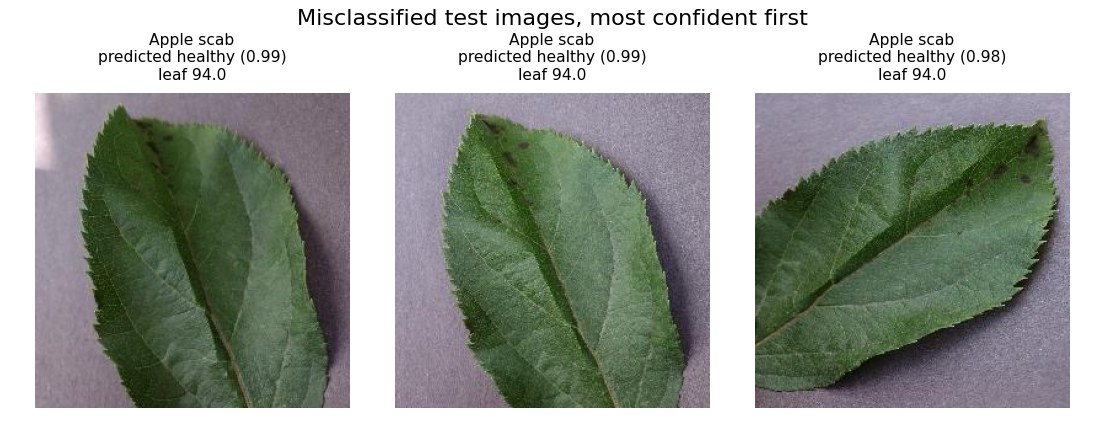
\includegraphics[width=0.70\textwidth]{mobilenet_leaf_test_errors.jpg}
\caption{Every misclassified test image, most confident first. All three are the same
leaf: a few small dark scab lesions near the tip and margin on otherwise unbroken green
tissue.}
\end{figure}

Five of that leaf's photographs are in the test set. The model calls three healthy with
high confidence, and gets the other two right --- one of them only marginally, at 0.52.

\textbf{A hypothesis tested and rejected.} Because the lesions sit near the leaf margin,
the deterministic centre crop might have been discarding them. Re-running all five
images through a full-frame resize that crops nothing changed \emph{none} of the five
predictions. The centre crop is therefore not the mechanism. The more likely reading is
simply that sparse, small lesions on predominantly healthy tissue do not produce enough
evidence for this model --- offered as a reading of the evidence, not a conclusion, since
it was not itself tested further.

\textbf{The confidence figures matter more than the error count.} Mean confidence on the
wrong predictions is 0.9901, the maximum 0.9940, so the 0.70 threshold the API uses to
flag uncertain results would have caught \textbf{0 of 3}. The model is confidently wrong,
and exposing a confidence score does not protect a user against that --- a limitation of
the mechanism, not a threshold needing tuning. No calibration was performed; a softmax
score is a model output, not a probability of being correct, and the interface is worded
accordingly: it says the model finds patterns consistent with a diseased leaf, never that
the leaf is diseased.

\section{System}

\textbf{Backend.} FastAPI served by uvicorn: a service description at the root, a
liveness probe at \texttt{/health}, a model description at \texttt{/model-info}, and the
classifier at \texttt{POST /predict}, taking a single multipart file field. Three
decisions are worth recording. The model loads once at startup, because building the
inference session costs far more than running it. The service depends on ONNX Runtime
rather than PyTorch, keeping the image near 150\,MB instead of approaching a gigabyte ---
decisive at 512\,MB of memory. Model-loading failures are recorded rather than raised, so
a missing model yields a degraded health response instead of a restart loop.

Uploads are validated on content type, emptiness, byte size against an 8\,MB limit and
decodability, with a further guard on pixel count so a decompression bomb cannot turn
one request into gigabytes of pixels. Internal errors are logged in full and returned as
a generic message. Responses use \texttt{400} for an undecodable image, \texttt{413} for
oversize, \texttt{415} for an unsupported type, \texttt{422} for a missing field and
\texttt{503} while the model is unavailable. A suite of 31 tests covers the split
invariants, the inference contract and each of those failure modes.

\textbf{Front end.} A small React application built with Vite. The workflow is linear:
select or drop an image, see it previewed, press one button, read the result. The result
panel shows the predicted label, the confidence, both class probabilities and a
plain-language message, with an explicit warning below the threshold. A model panel
reports architecture, classes, input size and threshold, fetched from the API rather
than duplicated in the interface. The theme is light and flat, with no gradients or
animation. A usage guide sits above the upload area so a first-time visitor learns what
the tool expects before choosing a file, and states plainly that anything other than an
apple leaf will still return a confident-looking answer that means nothing.

\begin{figure}[H]
\centering
\begin{subfigure}{0.54\textwidth}
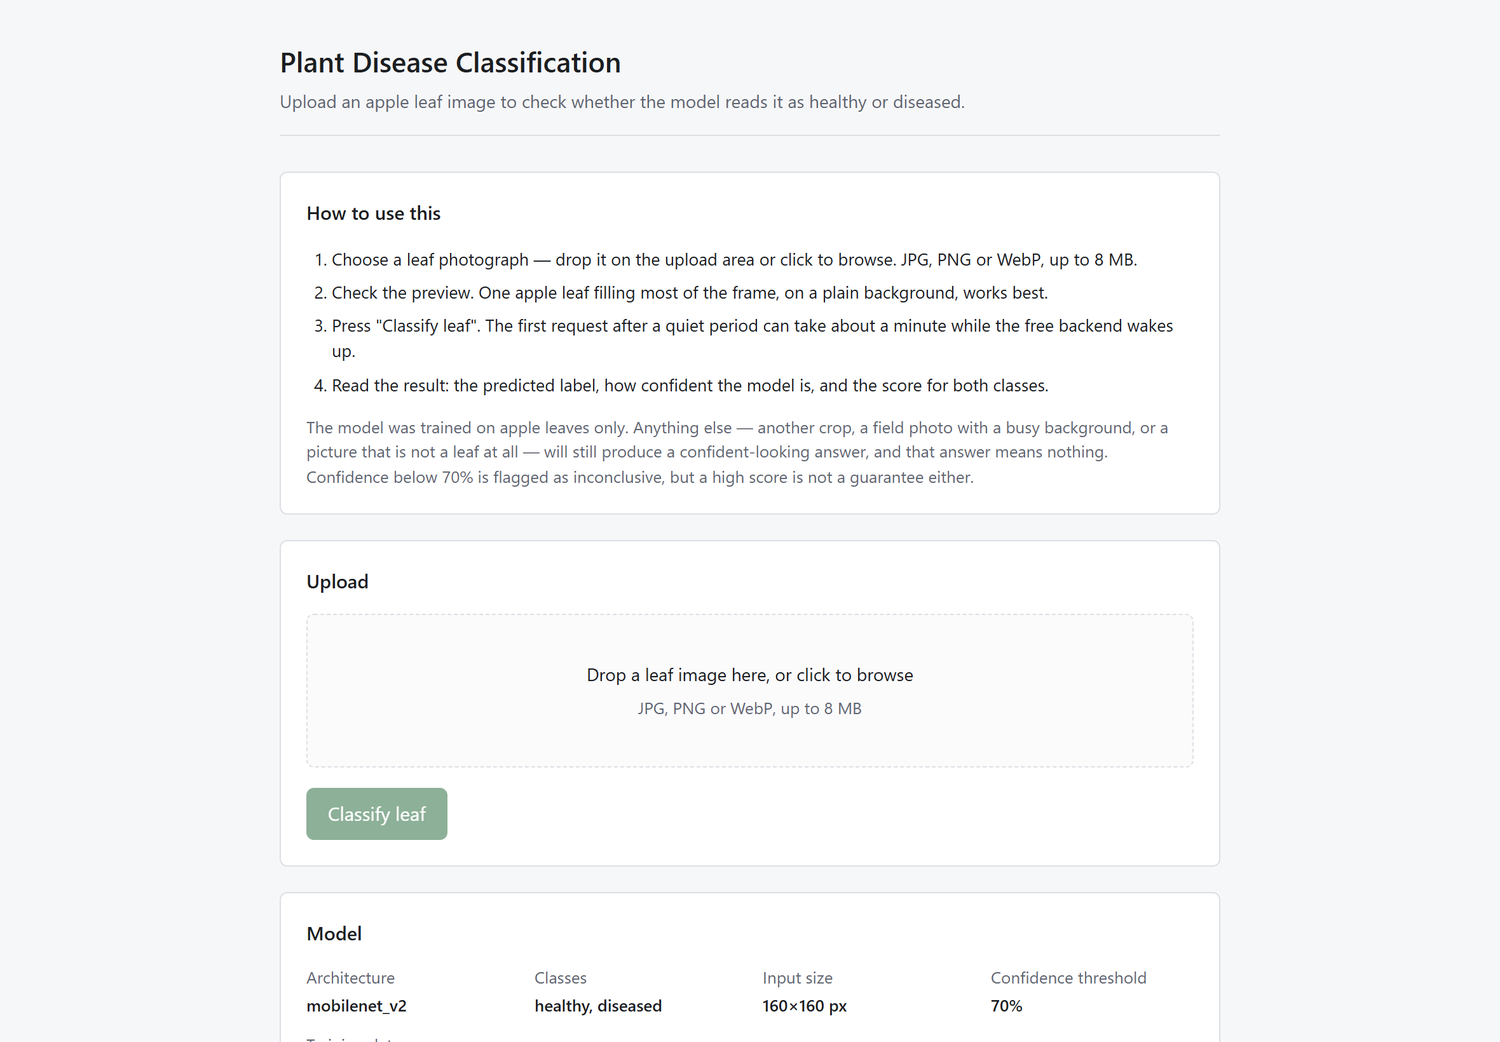
\includegraphics[width=\textwidth]{screenshot_upload.png}
\end{subfigure}\\[0.6em]
\begin{subfigure}{0.54\textwidth}
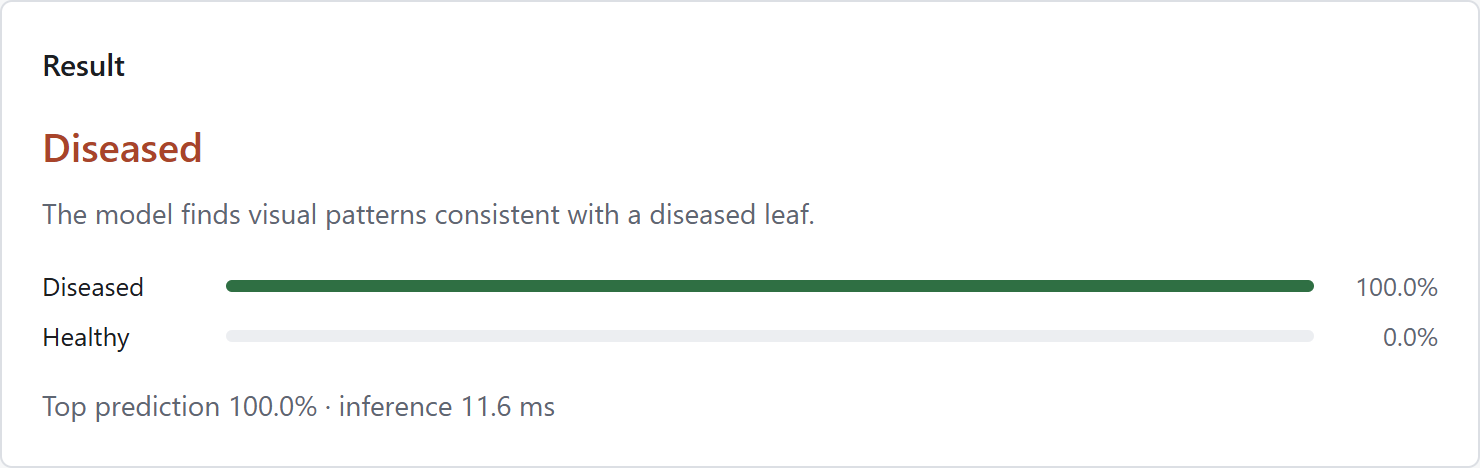
\includegraphics[width=\textwidth]{screenshot_result.png}
\end{subfigure}
\caption{The deployed interface: usage guide above the upload area, and the result panel
reporting both class scores and measured inference time.}
\end{figure}

\section{Deployment}
\label{sec:deployment}

The system deploys as two pieces: the inference API as a Docker web service on Render's
free tier, and the built front end as a static bundle on Vercel.

\begin{figure}[H]
\centering
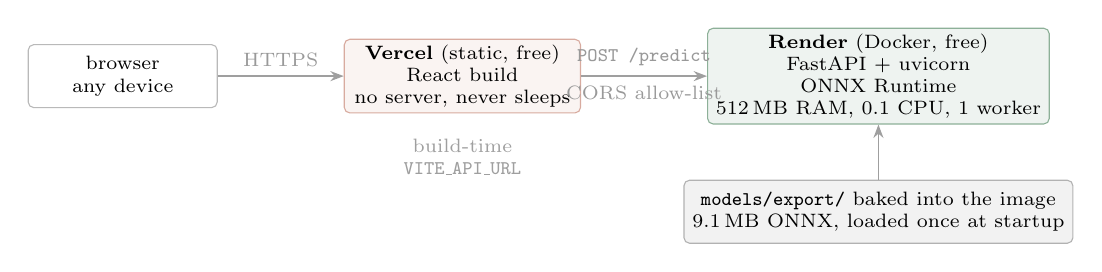
\begin{tikzpicture}[node distance=5mm and 9mm]

\node[pipebox, minimum width=24mm] (browser) {browser\\\scriptsize any device};

\node[servebox, right=16mm of browser, minimum width=30mm] (vercel)
  {\textbf{Vercel} (static, free)\\React build\\\scriptsize no server, never sleeps};

\node[trainbox, right=16mm of vercel, minimum width=34mm] (api)
  {\textbf{Render} (Docker, free)\\FastAPI + uvicorn\\ONNX Runtime\\%
   \scriptsize 512\,MB RAM, 0.1 CPU, 1 worker};

\node[pipebox, below=7mm of api, minimum width=34mm, fill=gray!10, draw=gray!60]
  (bundle2) {\texttt{models/export/} baked into the image\\%
             \scriptsize 9.1\,MB ONNX, loaded once at startup};

\draw[flow] (browser) -- node[above,font=\scriptsize,gray!80]{HTTPS} (vercel);
\draw[flow] (vercel) -- node[above,font=\scriptsize,gray!80]{\texttt{POST /predict}}
                        node[below,font=\scriptsize,gray!80]{CORS allow-list} (api);
\draw[flow] (bundle2) -- (api);

\node[font=\scriptsize, gray!75, below=2mm of vercel.south, align=center]
  {build-time\\\texttt{VITE\_API\_URL}};

\end{tikzpicture}
\caption{Deployment architecture. The two halves are hosted separately because their
constraints differ: the front end is static and always available, while the API needs a
container and is the piece that sleeps.}
\label{fig:architecture}
\end{figure}

Hugging Face Spaces was the original target and the Dockerfile still runs there
unchanged. It was ruled out by checking rather than assuming: as of 2026 the Hugging
Face documentation states that Gradio and Docker Spaces ``require a paid plan to
create'', with only static Spaces remaining free --- and a static Space cannot run the
model. That is exactly the kind of change that makes a free-tier assumption go stale.

The chosen tier's constraints shaped the implementation rather than being discovered
after it. The instance provides 512\,MB of memory and a fraction of a CPU core, which is
why the API serves ONNX and runs a single worker --- each worker would load its own copy
of the inference session. The exported model is a self-contained 9.1\,MB ONNX file whose
logits match the PyTorch original to $2.4\times10^{-6}$, and single-image inference on
one CPU thread measures \textbf{8.3\,ms}. The service sleeps after fifteen minutes idle
with a cold start near a minute, so the front end requests model information on load ---
which doubles as a wake-up call --- and allows a ninety-second timeout. Free instance
hours are capped at 750 per month, roughly one continuously running service.

\ifx\dashboardurl\empty
\textbf{Hosted URLs.} The deployment artefacts are complete and committed --- a
Dockerfile, a Render blueprint and step-by-step instructions --- but the hosted instance
runs under the author's own accounts and was not live when this document was generated.
No URL is quoted here rather than quote one that does not resolve.
\else
\textbf{Hosted URLs.} The dashboard is live at \href{\dashboardurl}{\texttt{\dashboardurl}}
and the API at \href{\apiurl}{\texttt{\apiurl}}. The first request after a quiet period
takes about a minute while the container starts.
\fi

\section{Challenges and how they were handled}

\begin{itemize}
\item \textbf{Spotting the leaf grouping at all.} The dataset card mentions it in
passing; the significance only appears on counting --- 3{,}171 images from 505 leaves.
The response was to build the split on leaf identity, audit the official split against
the same rule, and assert the property in the test suite so it cannot regress silently.
\item \textbf{A saturated benchmark.} With validation macro F1 at 1.0000 from the third
epoch, neither the architecture choice nor the leakage demonstration could be settled on
validation accuracy. Leakage was therefore measured structurally and the architecture
chosen on measured deployment cost, both reported as such rather than dressed up as
accuracy findings.
\item \textbf{Training on a laptop CPU.} Benchmarking showed the model step, not the
data loader, was the bottleneck --- roughly 127\,s per epoch against 13 --- so the fix
was 160-pixel inputs and two loader workers rather than four, leaving the physical cores
to the backward pass instead of competing with it.
\item \textbf{The deployment target disappeared mid-project}, as described above.
\item \textbf{A silently split model export.} PyTorch wrote the ONNX weights to a
sidecar file once they passed its size threshold. It loaded correctly in place and would
have failed only after someone copied the graph without it, so the export step now folds
the weights back into a single self-contained file and a test runs the shipped bundle
over the whole test split to confirm it still scores what the report claims.
\end{itemize}

\section{Limitations}

\begin{itemize}
\item \textbf{The benchmark is close to saturated.} Validation macro F1 reaches 1.0000
by the third epoch, which says more about the dataset than the model, and model
selection therefore picks the first epoch to hit the ceiling rather than a demonstrably
better checkpoint. Read the 99.51\% in that light.
\item \textbf{PlantVillage is a laboratory dataset.} Leaves are detached and
photographed against uniform backgrounds under controlled lighting, and published work
has repeatedly found such models degrade sharply on field photographs. Nothing here
contradicts that; nothing here measures it either.
\item \textbf{Apple only, with no out-of-distribution detection.} The model still
returns a confident answer for a tomato leaf, a hand or a wall, because a two-class
softmax has nowhere else to put its mass.
\item \textbf{The effective sample size is 505 leaves, not 3{,}171 images.} The image
count flatters the independent evidence behind every figure here.
\item \textbf{Confidence is uncalibrated} and, as shown above, can be wrong at 0.99.
\item \textbf{The binary output hides which disease is present} --- what the brief asked
for, but scab, black rot and cedar apple rust warrant different responses.
\end{itemize}

\section{Future work}

The most valuable next step is evaluation on field imagery --- PlantDoc or a similar
in-situ dataset --- to measure the laboratory-to-field gap rather than leaving it as a
caveat; everything else is secondary to knowing that number. After it: temperature
scaling with a rejection option, so out-of-distribution uploads can be declined instead
of labelled; keeping the four-way disease head alongside the binary one, since the
labels already carry that information; Grad-CAM overlays to check the model attends to
lesions rather than to background, which would also test the reading offered above; and
group-aware cross-validation over all 505 leaves, to report intervals rather than point
estimates.

\section{Conclusion}

The system meets the brief: a transfer-learned classifier, a validated API, a light web
interface and a deployment path onto free infrastructure, with accuracy, precision,
recall, F1 and a confusion matrix on a genuinely held-out test set.

The judgement worth carrying forward is not the 99.51\% figure. It is that this dataset
holds 6.3 photographs of each physical leaf, that a conventional random split therefore
leaks 100\% of validation images, and that the resulting score would have looked
slightly better while meaning considerably less. The number reported here is lower than
a leaky pipeline would have produced, and it is the one that can be defended.

\begin{thebibliography}{9}\small
\bibitem{mohanty2016}
S.~P. Mohanty, D.~P. Hughes and M.~Salath\'e,
``Using deep learning for image-based plant disease detection,''
\emph{Frontiers in Plant Science}, vol.~7, 2016.
\href{https://doi.org/10.3389/fpls.2016.01419}{doi:10.3389/fpls.2016.01419}
\bibitem{dataset}
PlantVillage dataset (colour configuration), Hugging Face Hub.
\href{https://huggingface.co/datasets/mohanty/PlantVillage}{huggingface.co/datasets/mohanty/PlantVillage}
\end{thebibliography}

\end{document}
